

\begin{frame}
\frametitle{1D PPM Model Base Case I}
\begin{figure}[ht]
\begin{minipage}[b]{0.45\linewidth}

  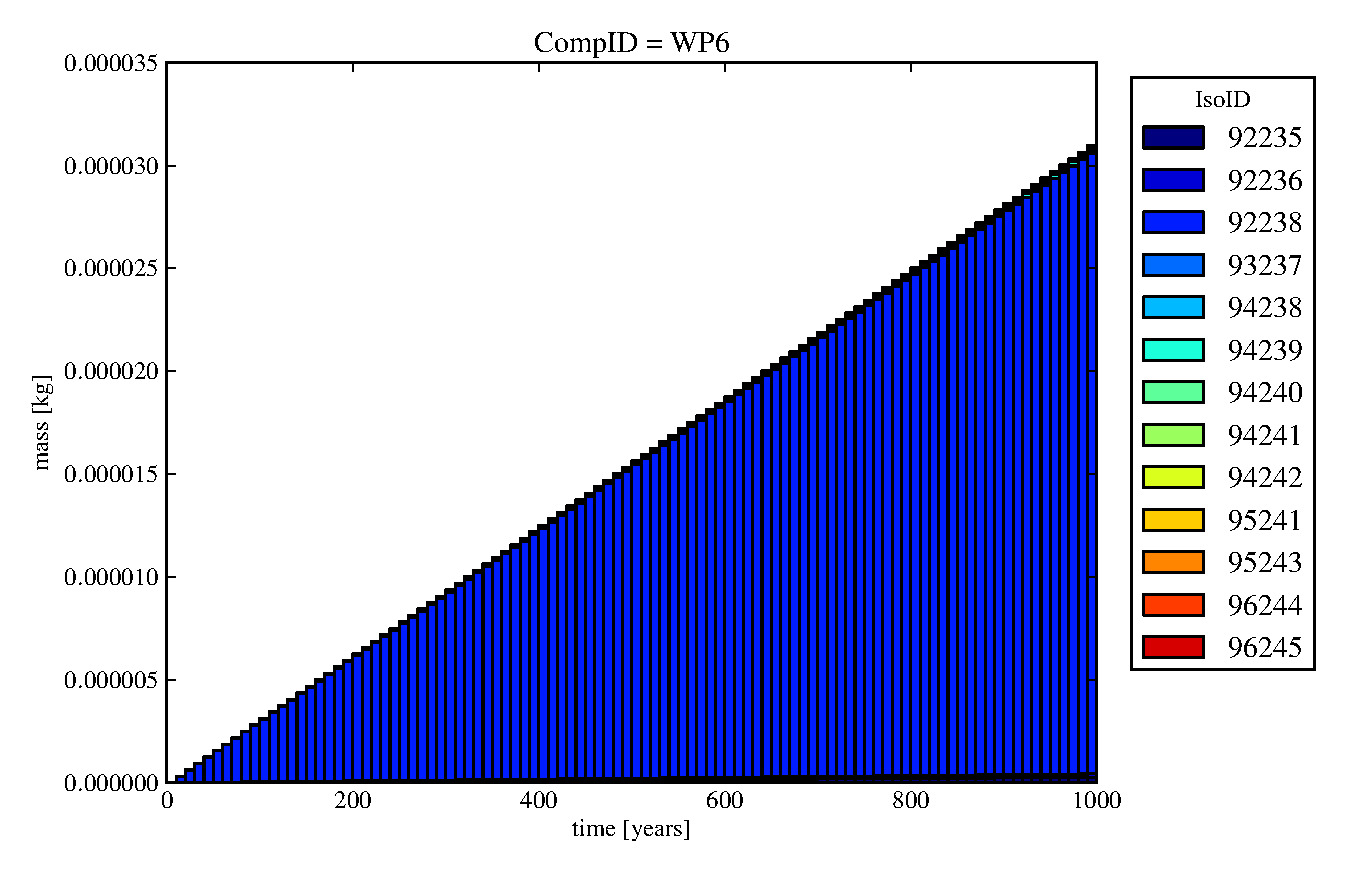
\includegraphics[width=0.8\textwidth]{./images/od2.eps}
  \caption[Case ODI Waste Form Contaminants.]{
    WF 5 slowly releases material into WP 6.
    }
  \label{fig:drIVwf5}
  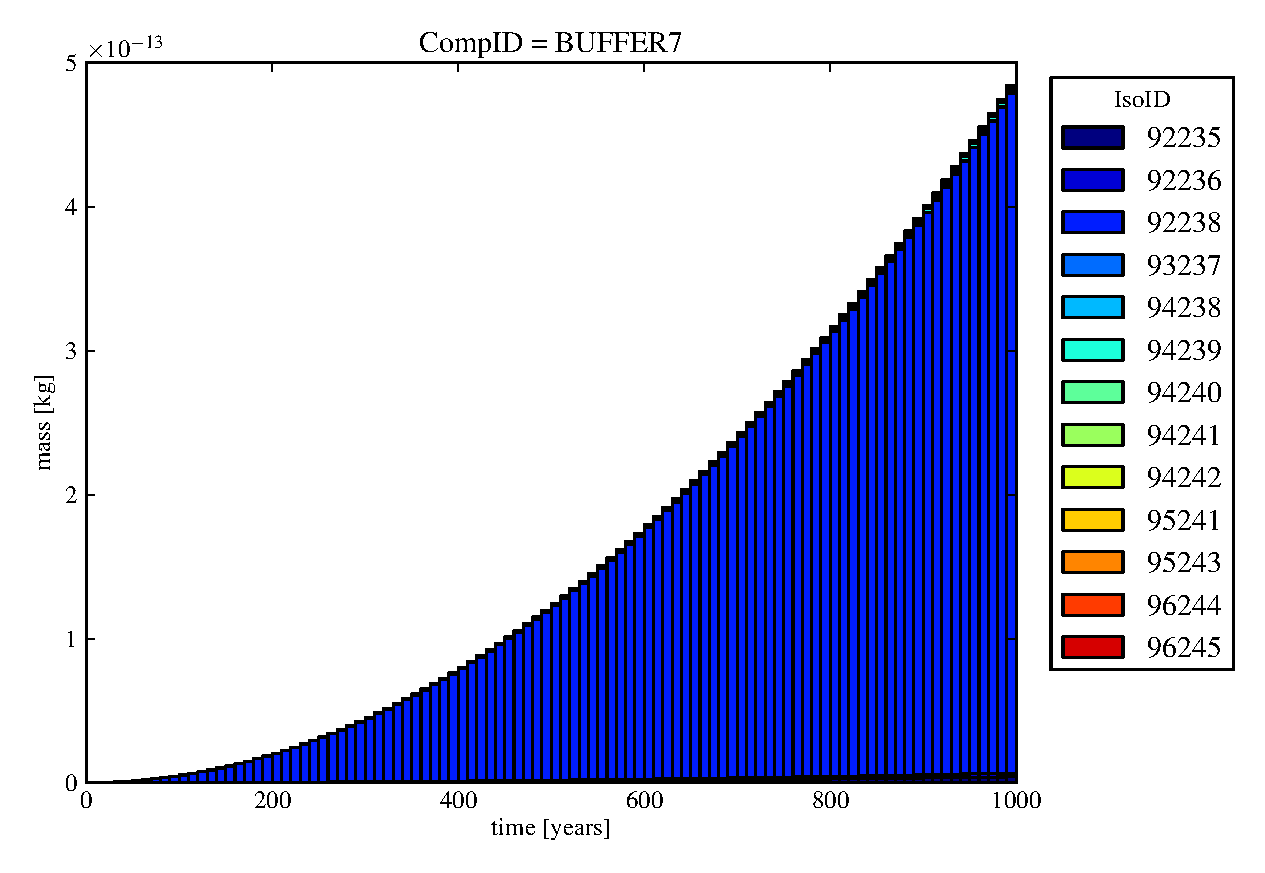
\includegraphics[width=0.8\textwidth]{./images/od3.eps}
  \caption[Case ODI Buffer Contaminants]{
    Buffer 7 slowly receives and releases material.
    }
  \label{fig:drIVbuff}
\end{minipage}
\hspace{0.05\linewidth}
\begin{minipage}[b]{0.45\linewidth}
  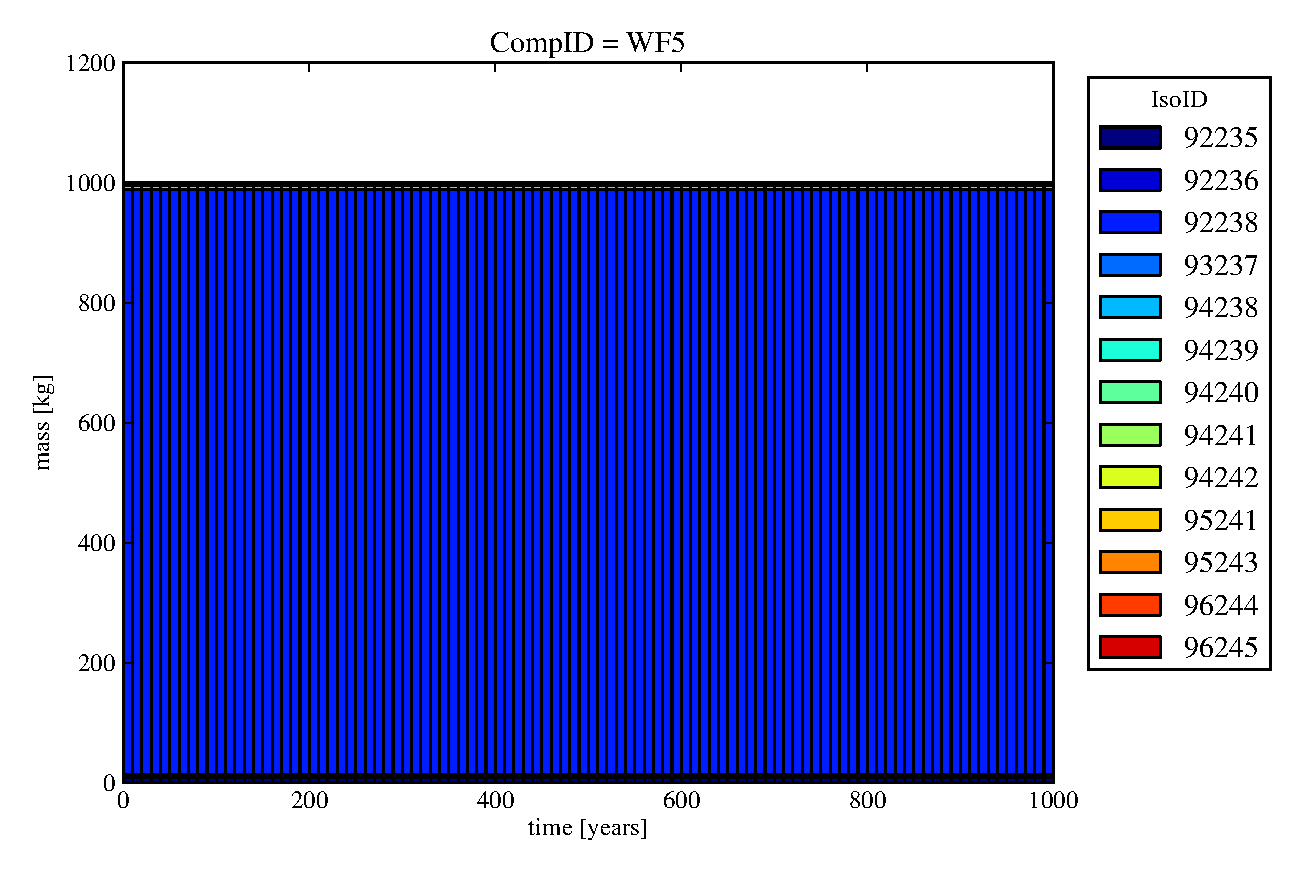
\includegraphics[width=0.8\textwidth]{./images/od1.eps}
  \caption[Case ODI Waste Package Contaminants.]{ 
    Waste Package 6 slowly receives and releases material. 
    }
  \label{fig:drIVwp6}
  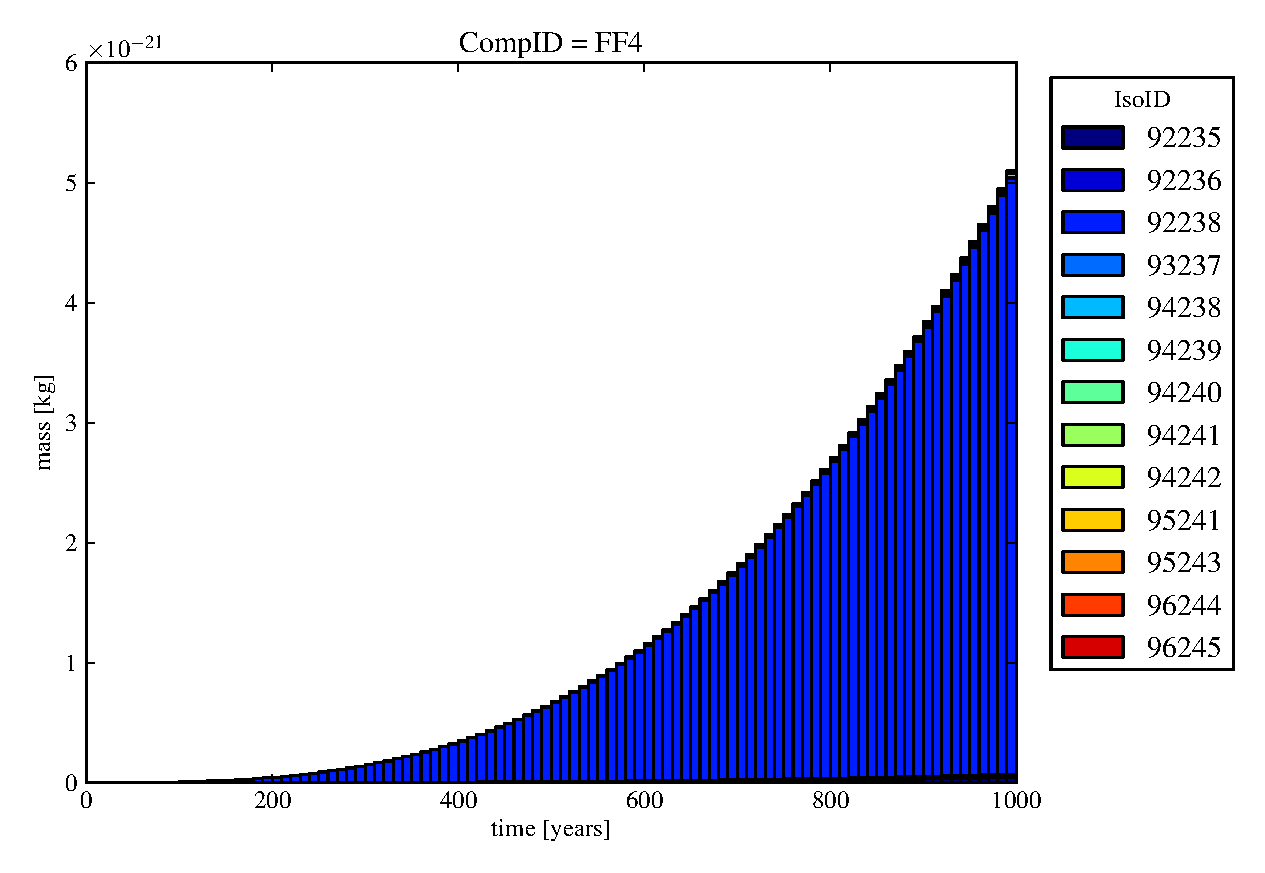
\includegraphics[width=0.8\textwidth]{./images/od0.eps}
  \caption[Case ODI Waste Package Contaminants.]{ 
    Far Field 4 acheives total containment.
    }
  \label{fig:drIVff0}


  \end{minipage}
\end{figure}
\end{frame}

\begin{frame}
\frametitle{1D PPM Model Base Case I}
\begin{figure}[ht]
\centering
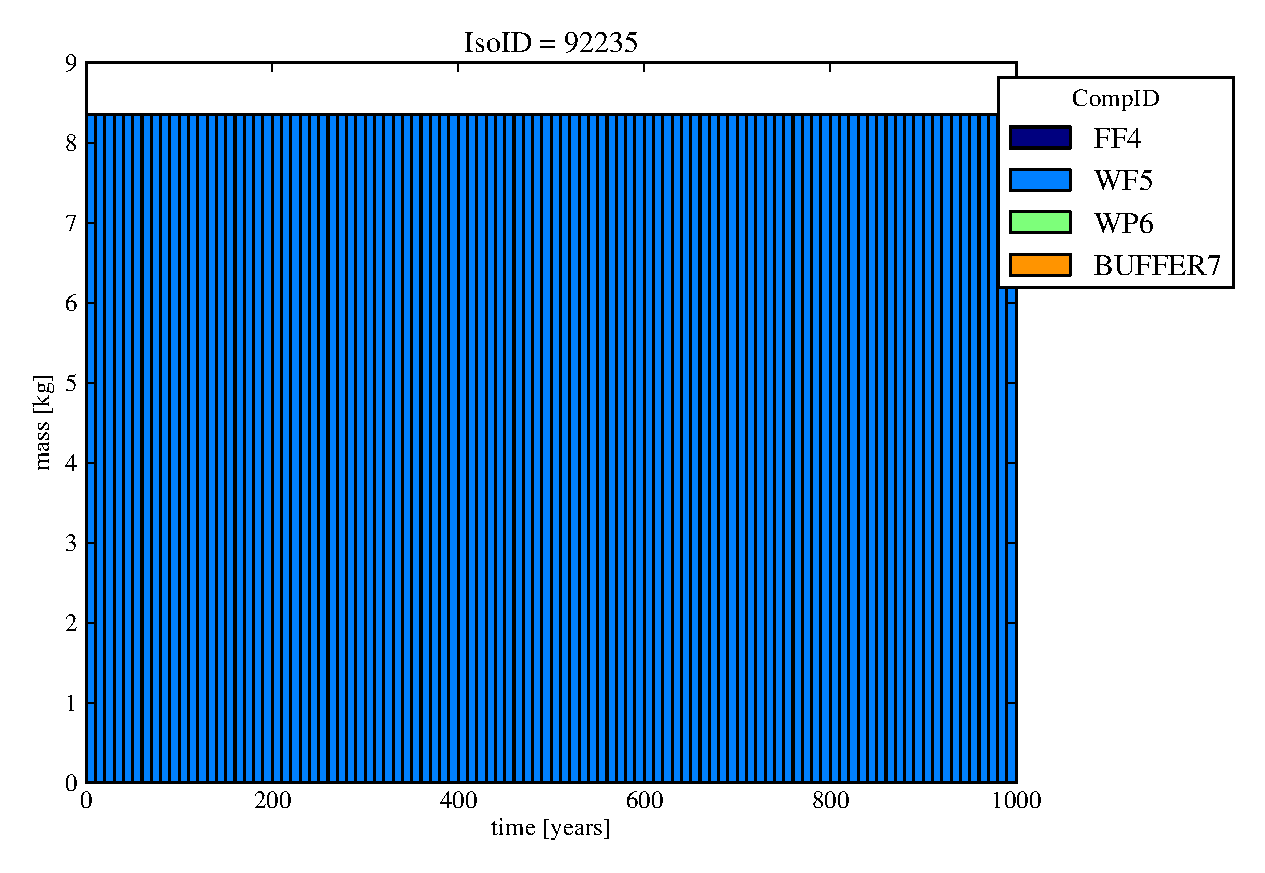
\includegraphics[width=0.8\textwidth]{./images/od.eps}
\caption[1 Dimensional PPM Model.]{
For the case in which transport through all components is represented by the 1 
Dimensional PPM model, material moves very slowly into the far field. 
}
\label{fig:odall}
\end{figure}
\end{frame}

